\documentclass[aspectratio=169]{beamer}
\usetheme[faculty=phil]{fibeamer}
\usepackage{polyglossia}
\setmainlanguage{english} %% main locale instead of `english`, you
%% can typeset the presentation in either Czech or Slovak,
%% respectively.
\setotherlanguages{russian} %% The additional keys allow
%%
%%   \begin{otherlanguage}{czech}   ... \end{otherlanguage}
%%   \begin{otherlanguage}{slovak}  ... \end{otherlanguage}
%%
%% These macros specify information about the presentation
\title[AGLA2]{Analytical Geometry and Linear Algebra II, Lab 10} %% that will be typeset on the
\subtitle{Fast Fourier Transform (FFT) \\ Discrete Fourier Transform (DFT) \\ Circulant Matrix
         } %% title page.
\author{Oleg Bulichev}
%% These additional packages are used within the document:
\usepackage{ragged2e}  % `\justifying` text
\usepackage{booktabs}  % Tables
\usepackage{tabularx}
\usepackage{tikz}      % Diagrams
\usetikzlibrary{calc, shapes, backgrounds}
\usepackage{amsmath, amssymb}
\usepackage{url}       % `\url`s
\usepackage{listings}  % Code listings
% \usepackage{subfigure}
\usepackage{floatrow}
\usepackage{subcaption}
\usepackage{mathtools}
\usepackage{todonotes}
\usepackage{fontspec}
\usepackage{multicol}
\usepackage{pdfpages}
\usepackage{wrapfig}
\usepackage{animate}

\graphicspath{{resources/}}
\frenchspacing

\setbeamertemplate{caption}[numbered]
\usetikzlibrary{graphs}

% \usepackage[backend=biber,style=ieee,autocite=footnote]{biblatex}
% \addbibresource{biblio.bib}
% \DefineBibliographyStrings{english}{%
%   bibliography = {References},}

\newcommand{\oleg}[2][] {\todo[color=red, #1] {OLEG:\\ #2}}
\newcommand{\fbckg}[1]{\usebackgroundtemplate{\includegraphics[width=\paperwidth]{#1}}}%frame background

\usepackage[framemethod=TikZ]{mdframed}
\newcommand{\dbox}[1]{
\begin{mdframed}[roundcorner=3pt, backgroundcolor=yellow, linewidth=0]
\vspace{1mm}
{#1}
\vspace{1mm}
\end{mdframed}
}

\begin{document}
\setlength{\abovedisplayskip}{0pt}
\setlength{\belowdisplayskip}{0pt}
\setlength{\abovedisplayshortskip}{0pt}
\setlength{\belowdisplayshortskip}{0pt}

\fbckg{fibeamer/figs/title_page.png}
\frame[c]{\setcounter{framenumber}{0}
    \usebeamerfont{title}%
    \usebeamercolor[fg]{title}%
    \begin{minipage}[b][6.5\baselineskip][b]{\textwidth}%
        \textcolor{black}{\raggedright\inserttitle}
    \end{minipage}
    % \vskip-1.5\baselineskip

    \usebeamerfont{subtitle}%
    \usebeamercolor[fg]{framesubtitle}%
    \begin{minipage}[b][3\baselineskip][b]{\textwidth}
        \raggedright%
        \insertsubtitle%
    \end{minipage}
    \vskip.25\baselineskip
}
%   \frame[c]{\maketitle}

\fbckg{fibeamer/figs/common.png}


\begin{frame}[t]{Gilbert Strang's Goal VS My Goal}
\framesubtitle{}
\Large
    \begin{columns}[T,onlytextwidth]
        \begin{column}{0.49\textwidth}
            \textbf{Gilbert Strang's Goal} \\
            Is to give you a knowledge how to calculate Discrete Fourier Transform (DFT) by hand. It's an application for using Complex Numbers and Matrices.
        \end{column}
        \begin{column}{0.49\textwidth}
            \textbf{My Goal} \\ 
            Is to give you the application and the concept why do we need it. It won't be on the exam.
        \end{column}
    \end{columns}
\end{frame}


\begin{frame}[t]{Outline}
\framesubtitle{}
    \Large
    \begin{enumerate}
        \item Fourier Series, intuition
        \item From Fourier Series to DFT
        \item Fast Fourier Transform algorithm
    \end{enumerate}
\end{frame}

\begin{frame}[t]{How to imagine Fourier Transform}
    \framesubtitle{Video (rus)}
    \vspace{-0.6cm}
    \begin{figure}[H]
        \href{https://youtu.be/Vaa1BVGhpxI}{
            \centering
\includegraphics[height=6cm,width=1\textwidth,keepaspectratio]{wdwnfourier_rus.jpg}}
        % \caption{Click on a picture for a video}
        \label{fig:file_name}
    \end{figure}
\end{frame}

\begin{frame}[t]{How to sum up sines (Spectrum)}
    \framesubtitle{Video}
    \vspace{-0.6cm}
    \begin{figure}[H]
        \href{https://youtu.be/r18Gi8lSkfM}{
            \centering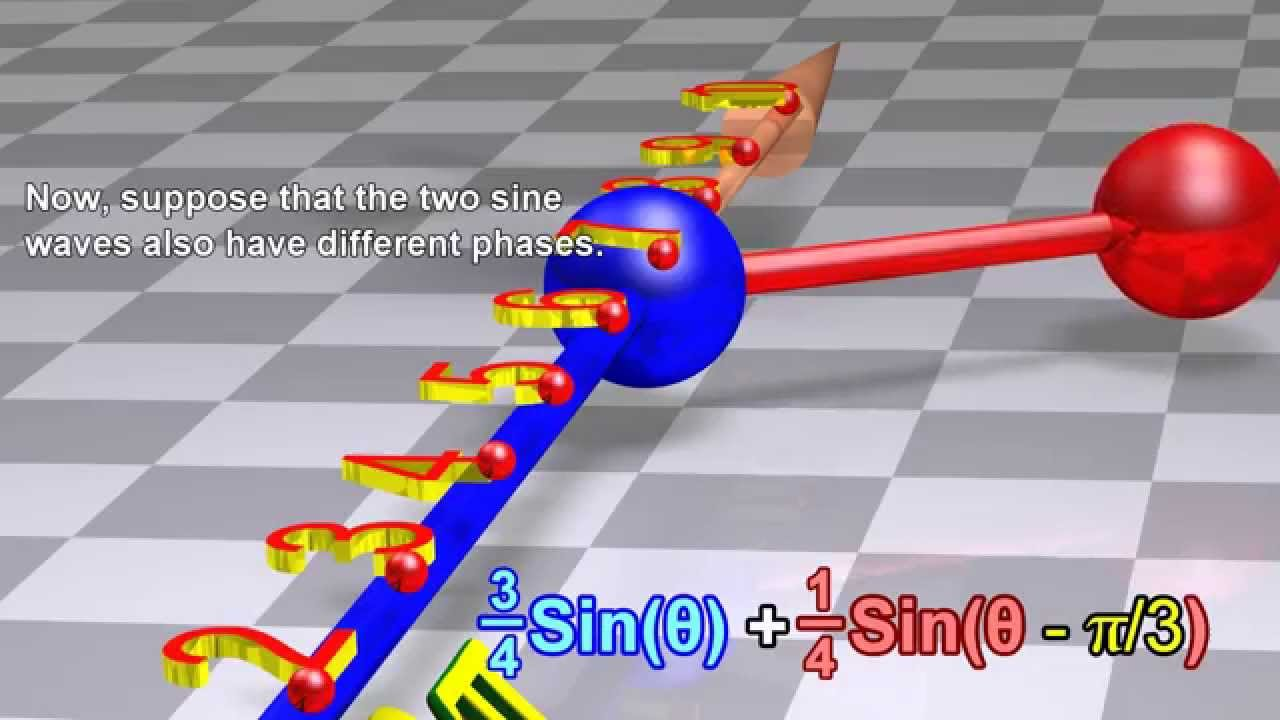
\includegraphics[height=6cm,width=1\textwidth,keepaspectratio]{Intro_to_fourier.jpg}}
        % \caption{Click on a picture for a video}
        \label{fig:Intro_to_fourier.jpg}
    \end{figure}
\end{frame}

\begin{frame}[t]{Draw pictures using Fourier Transform}
    \framesubtitle{Video}
    \vspace{-0.6cm}
    \begin{figure}[H]
        \href{https://youtu.be/r6sGWTCMz2k}{
            \centering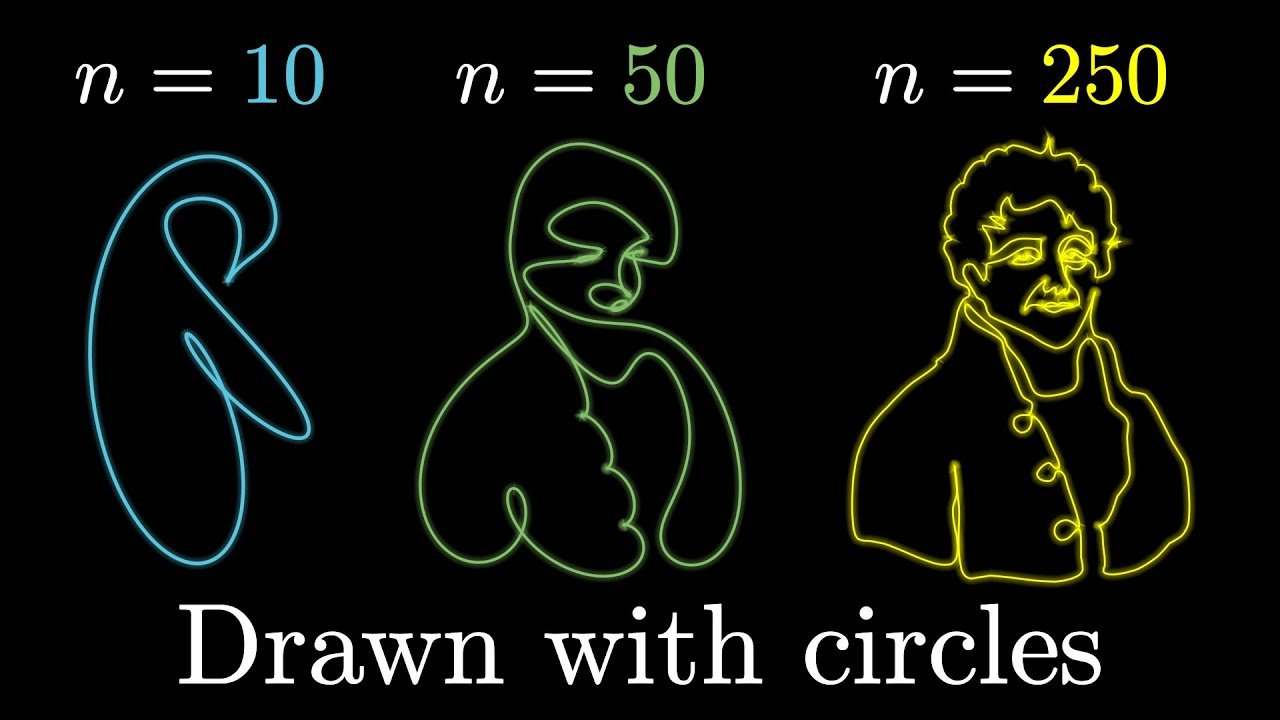
\includegraphics[height=6cm,width=1\textwidth,keepaspectratio]{drawn_with_circles.jpg}}
        % \caption{Click on a picture for a video}
        \label{fig:drawn_with_circles.jpg}
    \end{figure}
\end{frame}

\begin{frame}[t]{DFT: explanation using sound domain (watch at home)}
    \framesubtitle{Video}
    \vspace{-0.6cm}
    \begin{figure}[H]
        \href{https://youtu.be/spUNpyF58BY}{
            \centering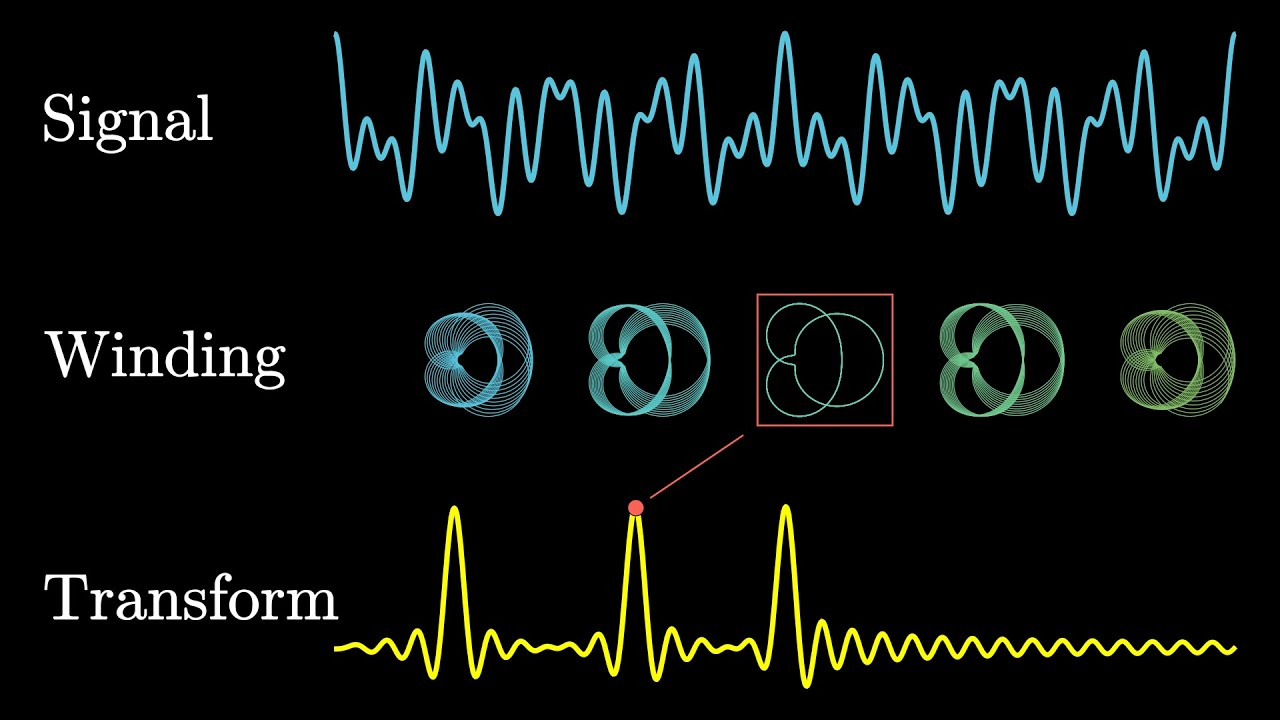
\includegraphics[height=6cm,width=1\textwidth,keepaspectratio]{fourier_sound.jpg}}
        % \caption{Click on a picture for a video}
        \label{fig:fourier_sound.jpg}
    \end{figure}
\end{frame}

\begin{frame}[t]{From Fourier Series to DFT}
\framesubtitle{}
\vspace{-0.75cm}
\begin{figure}[H]
    \centering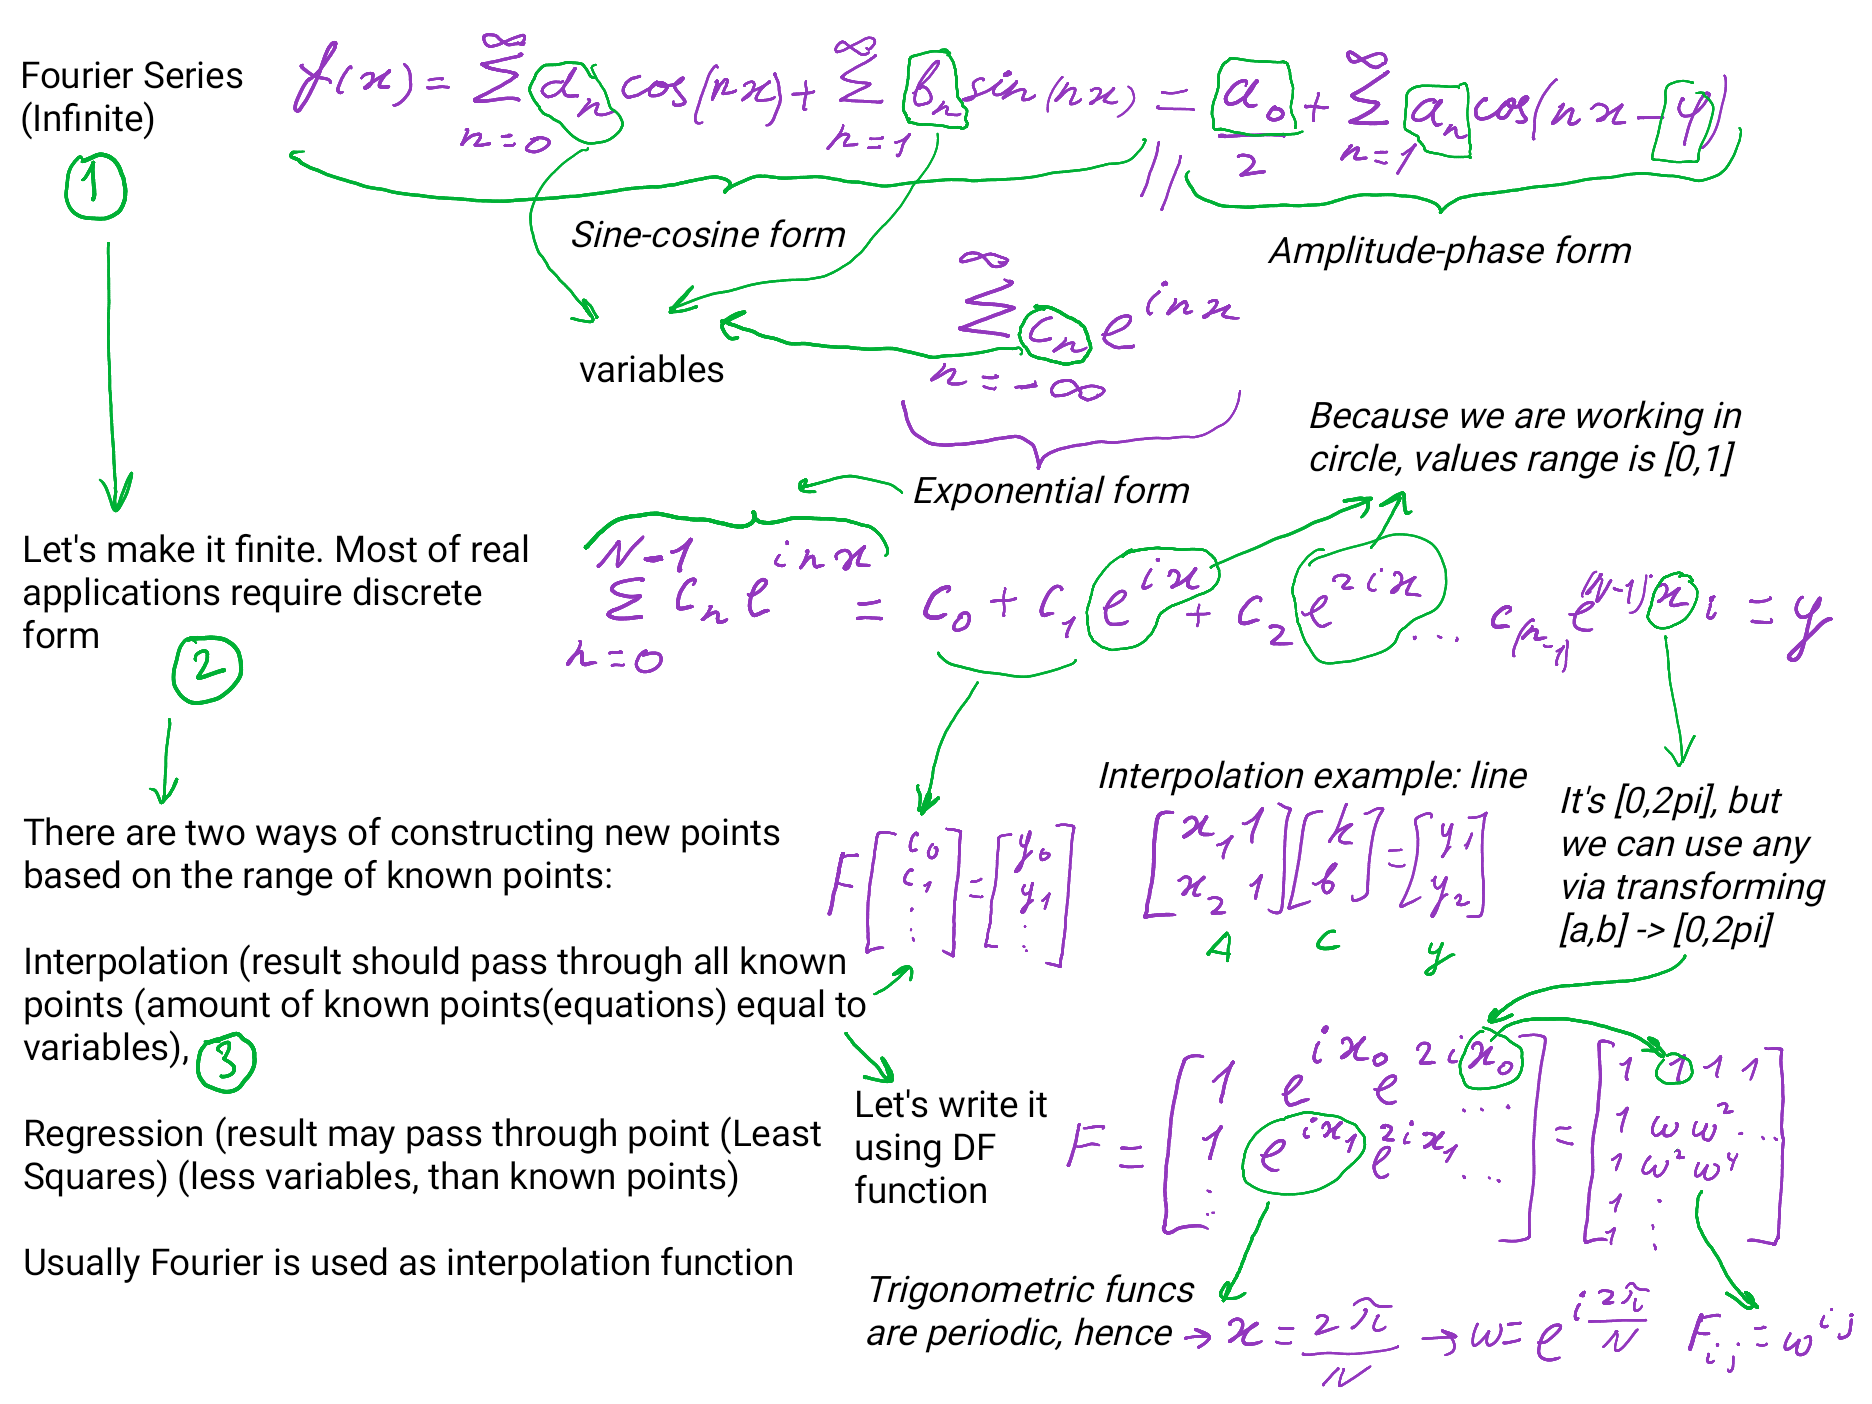
\includegraphics[height=7cm,width=1\textwidth,keepaspectratio]{AGLA2_for_slides_9.png}
    % \caption{caption_name}
    \label{fig:AGLA2_for_slides_9.png}
\end{figure}
\end{frame}

\usebackgroundtemplate{}
\setbeamercolor{background canvas}{bg=}
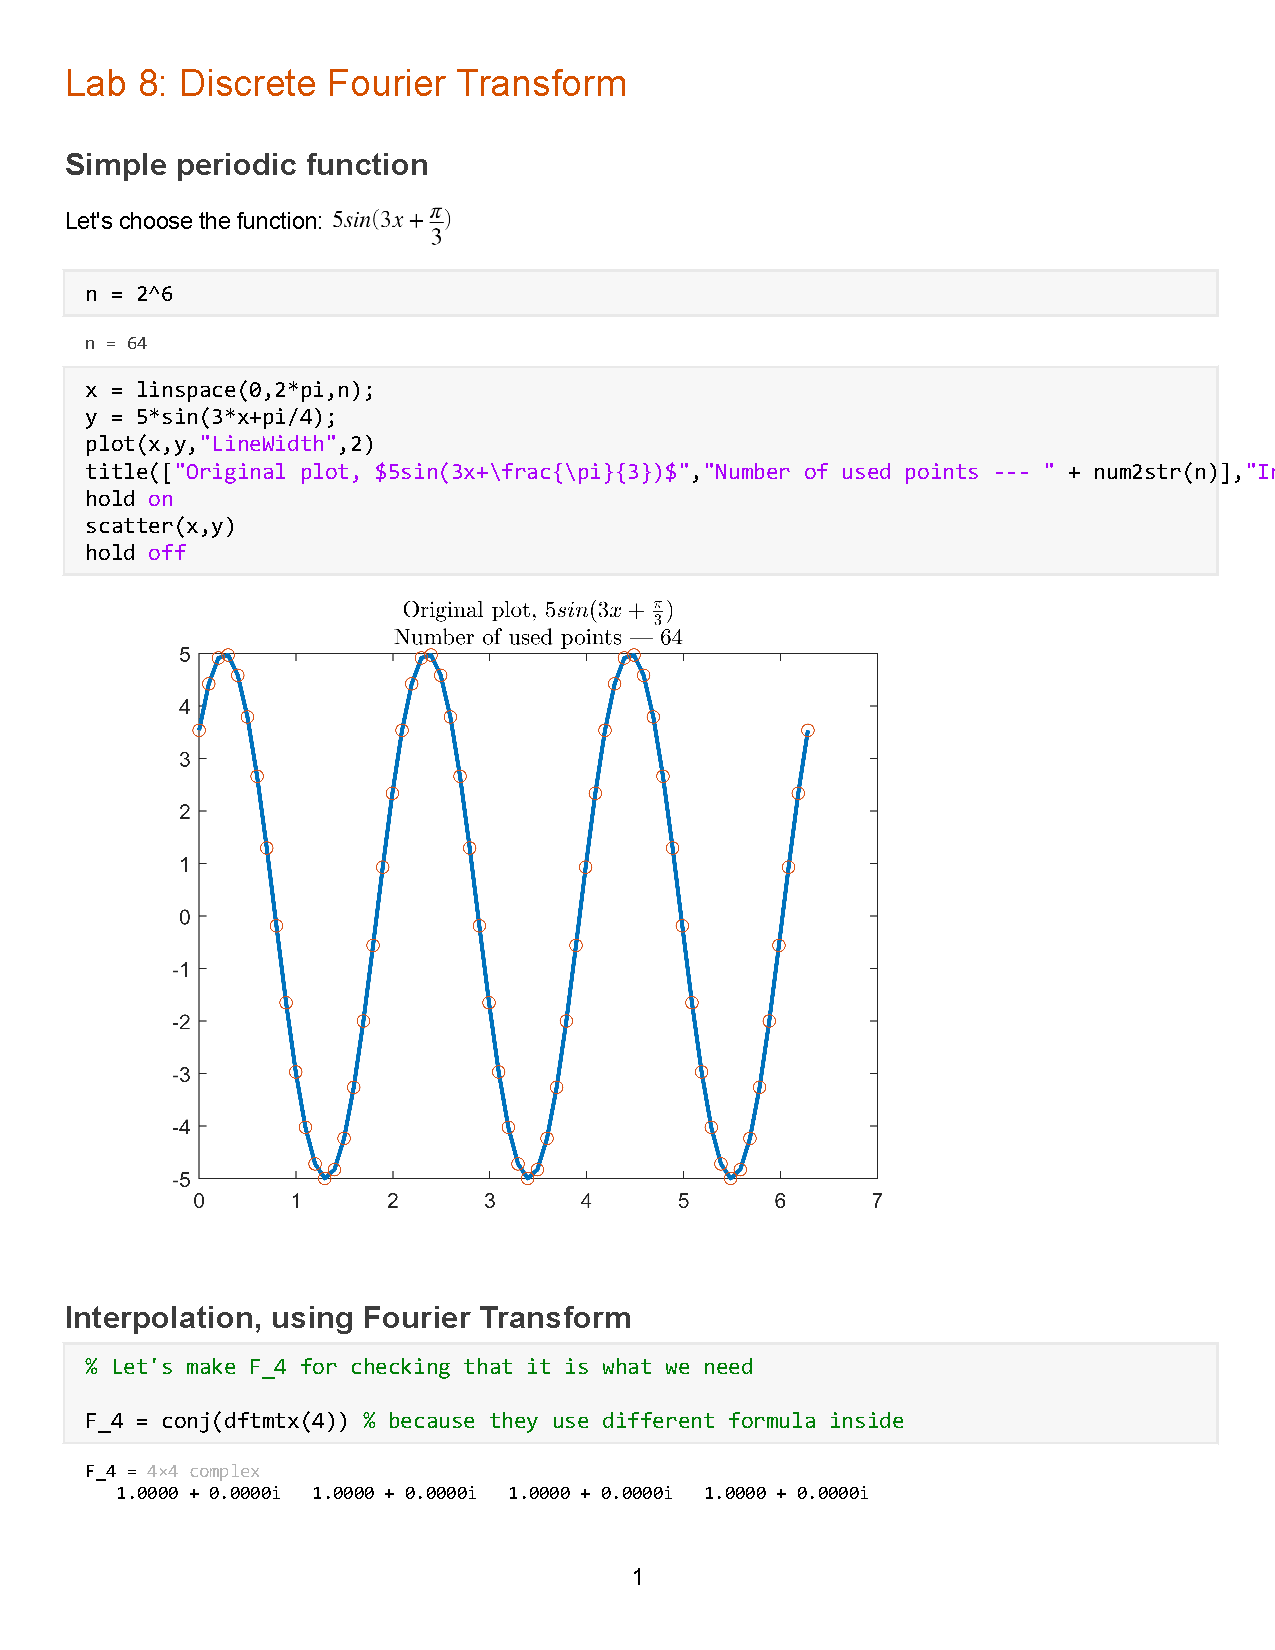
\includepdf[pages=-,fitpaper]{lab10.pdf}
\fbckg{fibeamer/figs/common.png}

\begin{frame}[t]{From Fourier Series to DFT}
    \framesubtitle{Properties}
    \vspace{-1.2cm}
    \begin{figure}[H]
        \centering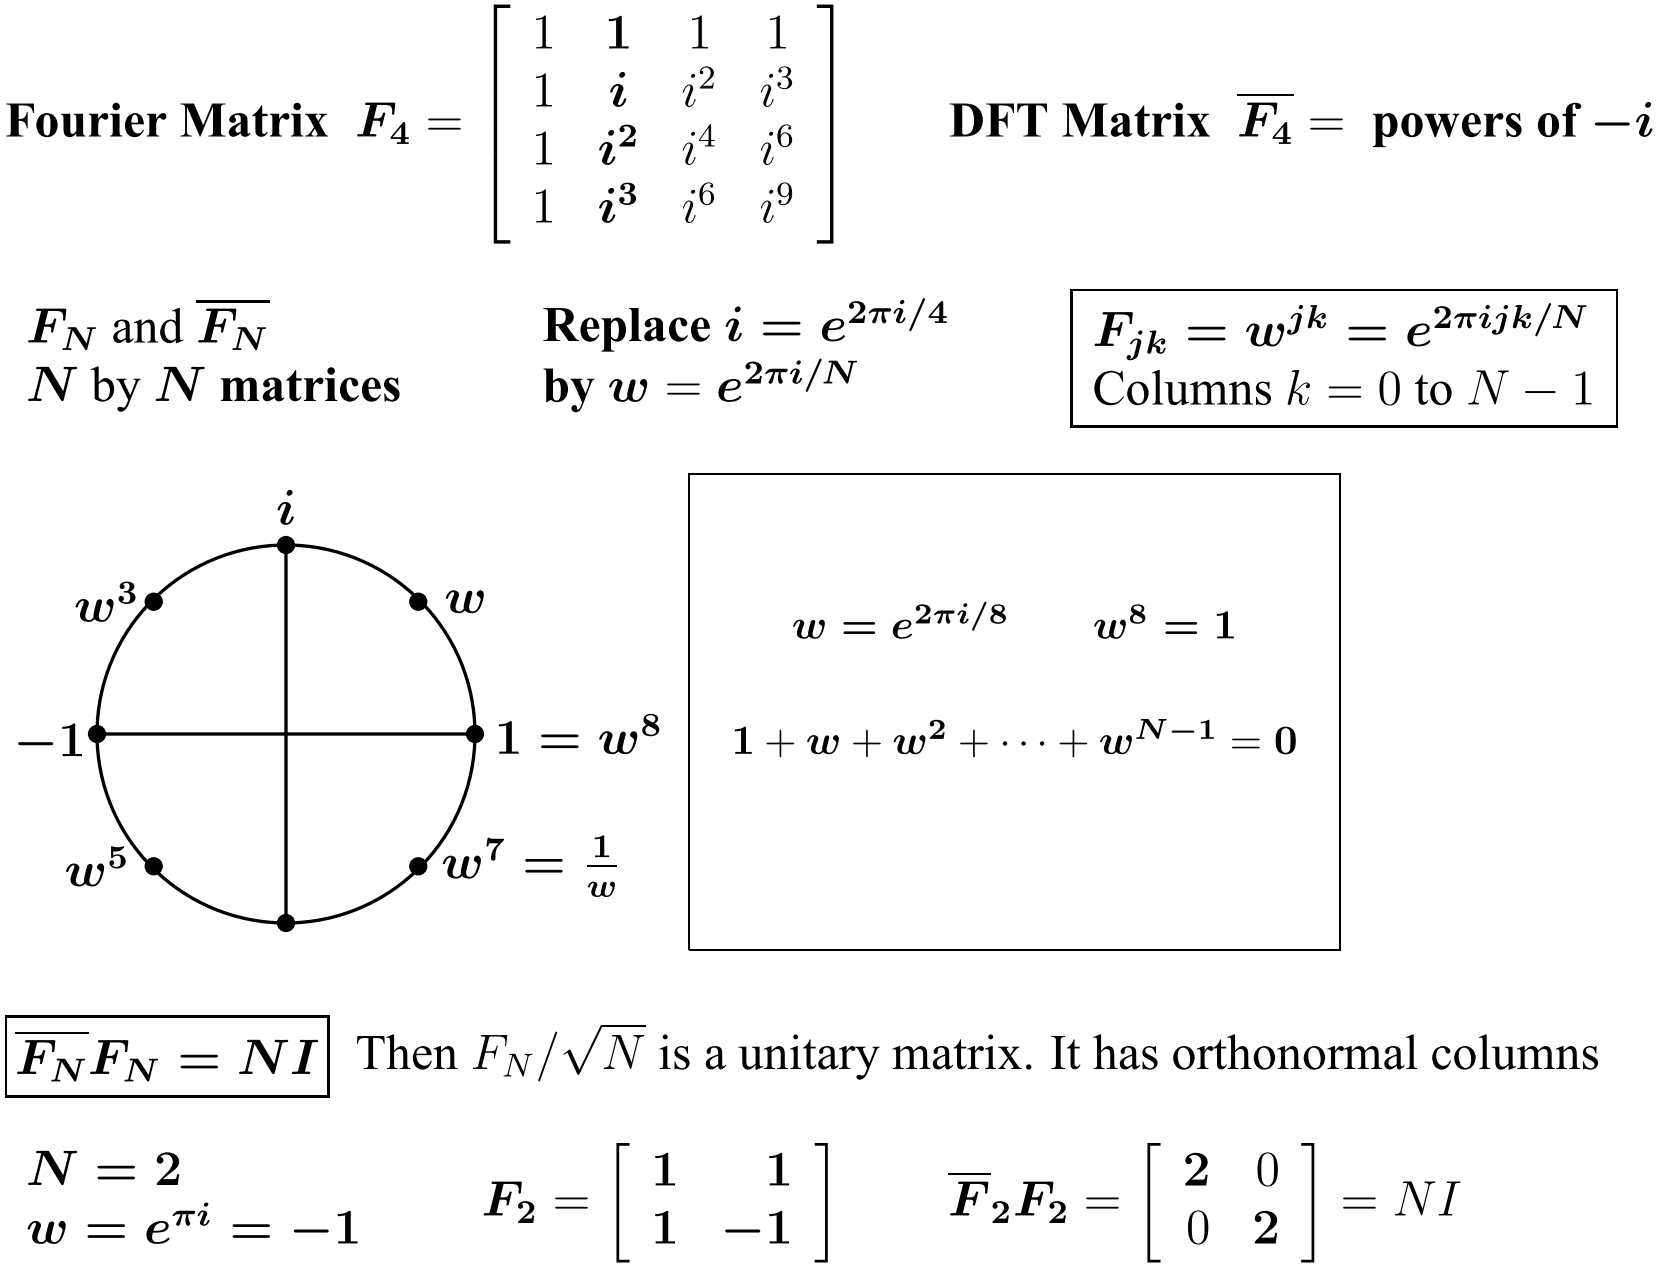
\includegraphics[height=6.8cm,width=1\textwidth,keepaspectratio]{DFT.png}
        % \caption{caption_name}
        \label{fig:DFT.png}
    \end{figure}
    \end{frame}

\begin{frame}[t]{DFT application: Sound (rus)}
    \framesubtitle{Video}
    \vspace{-0.6cm}
    \begin{figure}[H]
        \href{https://youtu.be/T0xlzPBdx6s?t=237}{
            \centering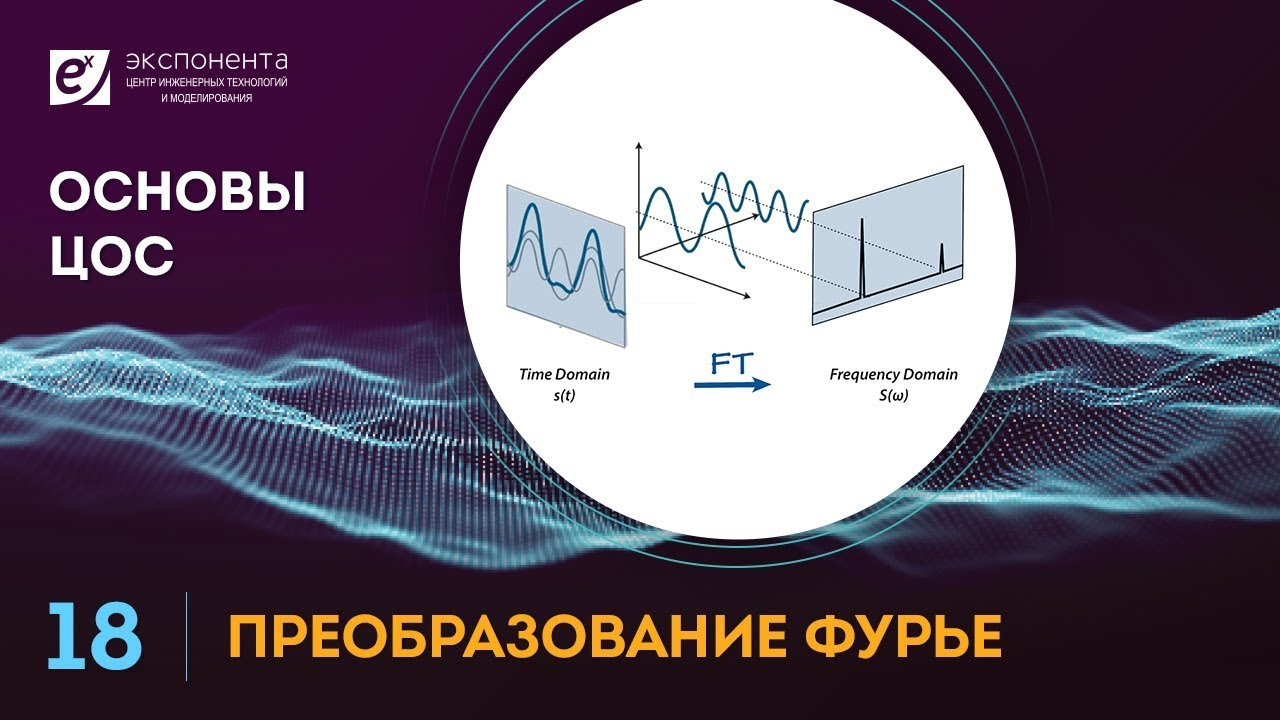
\includegraphics[height=6cm,width=1\textwidth,keepaspectratio]{fft_sound.jpg}}
        % \caption{Click on a picture for a video}
        \label{fig:fft_sound.jpg}
    \end{figure}
\end{frame}

\begin{frame}[t]{DFT application: Terrain Classification}
\framesubtitle{Feature Extraction step}
\vspace{-0.6cm}
\begin{columns}[T,onlytextwidth]
    \begin{column}{0.59\textwidth}
        \begin{block}{Problem}
            How to put such data (\ref{fig:Force_data_from_robot.png}) in ML algorithm (for instance SVM)?
        \end{block}
        \vspace{-0.5cm}
        \begin{figure}[H]
            \centering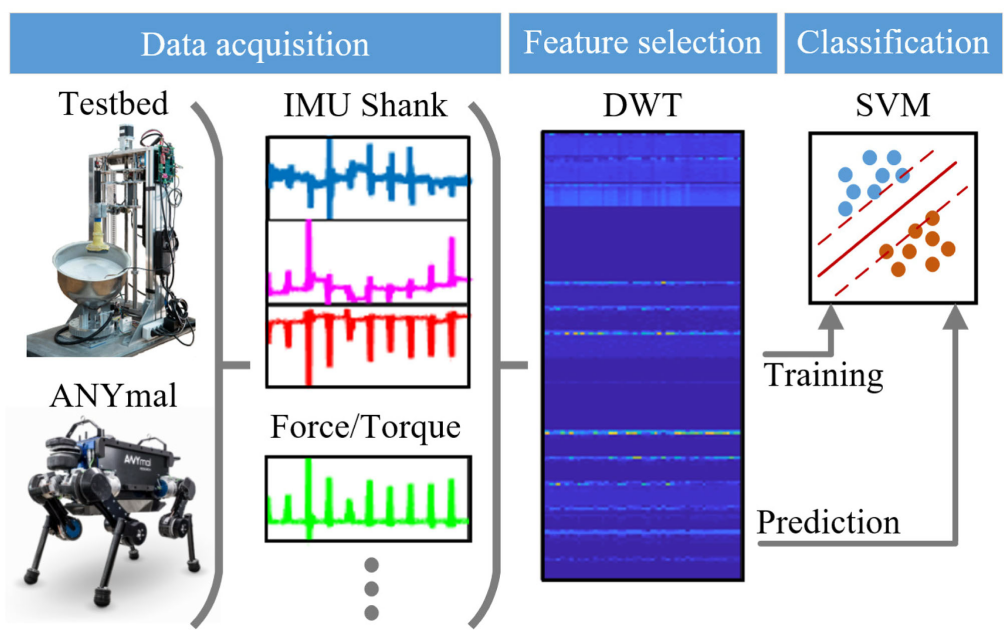
\includegraphics[height=4cm,width=1\textwidth,keepaspectratio]{TC_algo.png}
            % \caption{General approach for Terrain Classification}
            \label{fig:TC_algo.png}
        \end{figure}
    \end{column}
    \begin{column}{0.39\textwidth}
        \vspace{-0.75cm}
        \begin{figure}[H]
            \centering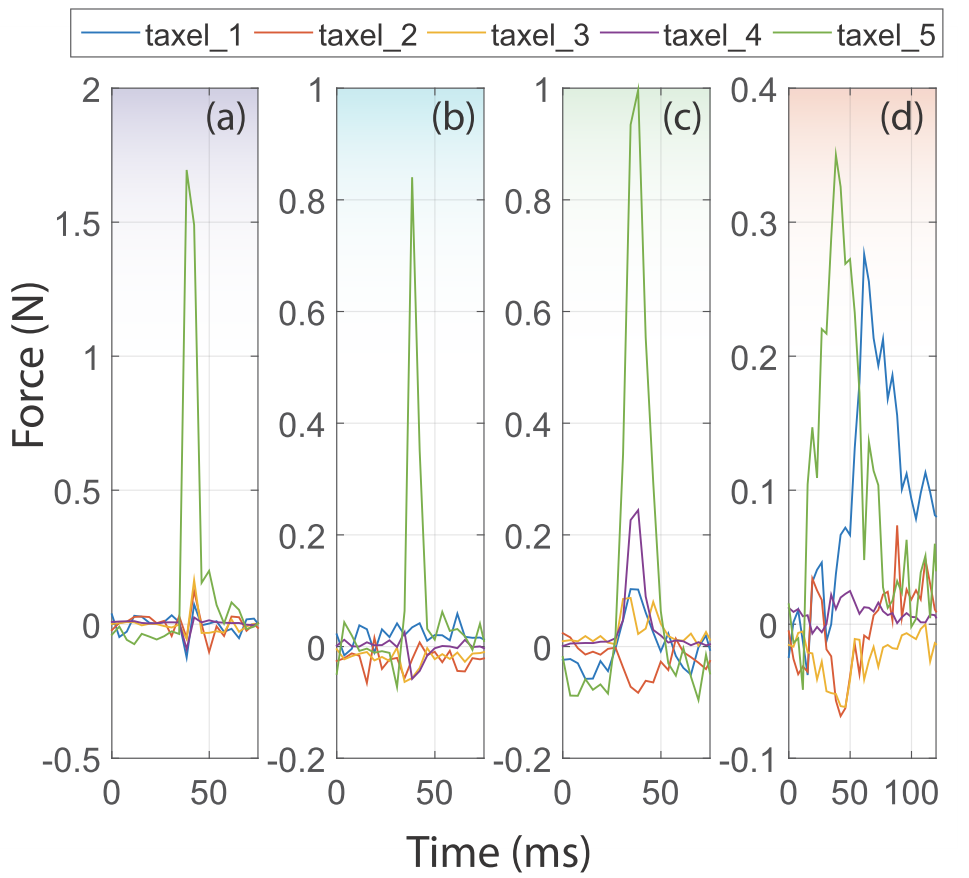
\includegraphics[height=6cm,width=1\textwidth,keepaspectratio]{Force_data_from_robot.png}
            \caption{Individual taxel forces recorded on different surfaces at 10 Hz stride frequency}
            \label{fig:Force_data_from_robot.png}
        \end{figure}
    \end{column}
\end{columns}
\end{frame}

\begin{frame}[t]{Fast Fourier Transform}
\framesubtitle{Problem Statement}
\Large
    Direct matrix multiplication of $\mathbf{c}$ by $F_N$ needs $\mathbf{N^2}$ multiplications. \\
    FFT factorization -- $\mathbf{\frac{1}{2}N\ log_2 N}$ multiplications. \\
    \textit{Benefit}: $N=2^{10}=1024$, $N^2 = 1$ million, FFT -- 5000 \\
    \textit{Constraint of FFT}: $N$ should be equal to $2^n$ \\
\end{frame}

\begin{frame}[t]{Fast Fourier Transform}
\framesubtitle{Algorithm}
\large
\vspace{-0.3cm}
\textbf{Step 1}: From 1024 to 512
\begin{equation*}
    \Bigg[\begin{matrix}
    F_{1024}  
    \end{matrix}\Bigg] = \begin{bmatrix}
    I & D\\ 
    I & -D 
    \end{bmatrix} \begin{bmatrix}
    F_{512} & 0\\ 
    0 & F_{512} 
    \end{bmatrix} \Bigg[\begin{matrix}
        P 
        \end{matrix}\Bigg],
\end{equation*}
where $D$ is a diagonal matrix of $F_{1024}$, but we took only half of it ($512x512$); \\
$P$ -- permutation matrix: for $P_{1024}$ puts columns 0,2,...,1022 ahead of 1,3,...1023. \\
\textit{Example: }$P_4=\begin{bmatrix}
1 & 0 & 0 & 0\\
0 & 0 & 1 & 0 \\ 
0 & 1  & 0 & 0 \\
0 & 0  & 0 & 1 
\end{bmatrix}$ \\ 
\textbf{Step 2}: From 512 to 256 \\
\textbf{Step 3...}: From 256 to 128 ... \textbf{Recursion} continues to small N: {$\mathbf{log_2 N}$} steps.
\end{frame}

\begin{frame}[t]{Task 1}
    \framesubtitle{}
    \vspace{-0.5cm}
    \begin{figure}[H]
        \centering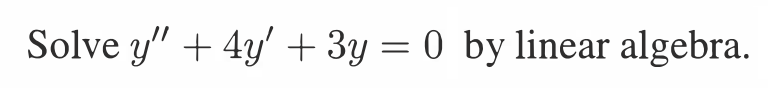
\includegraphics[height=3cm,width=1\textwidth,keepaspectratio]{4.png}
        % \caption{caption_name}
        \label{fig:4.png}
    \end{figure}
    \uncover<2->{
        \alert{\Large Answer} $D_{3,3}=e^{4\pi i/3}$ is also correct. It depend of $w$ equation (with minus or not).
        \begin{figure}[H]
            \centering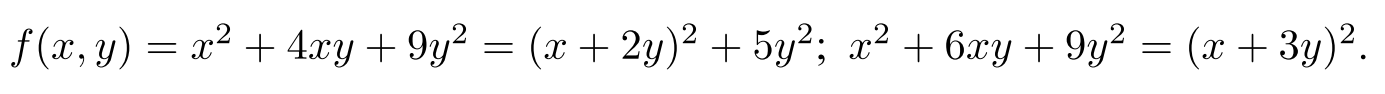
\includegraphics[height=2cm,width=1\textwidth,keepaspectratio]{4ans.png}
            % \caption{caption_name}
            \label{fig:4ans.png}
        \end{figure}
    }
\end{frame}

\begin{frame}[t]{Task 2}
    \framesubtitle{}
    \vspace{-0.5cm}
    \begin{figure}[H]
        \centering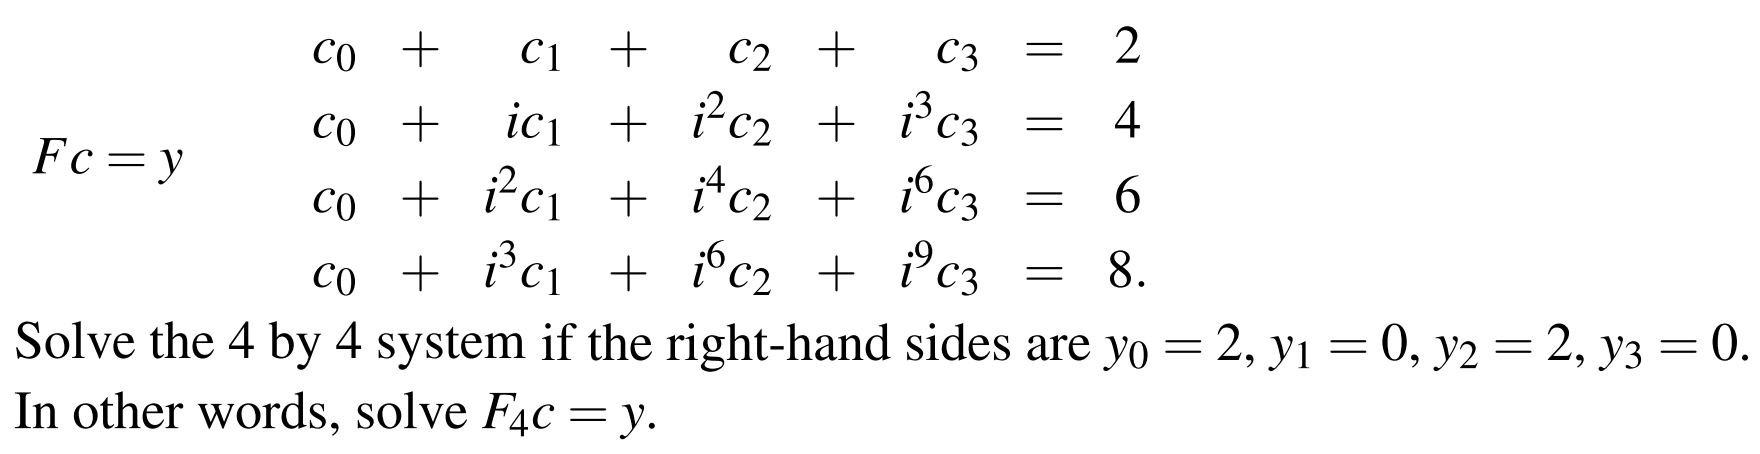
\includegraphics[height=3.5cm,width=1\textwidth,keepaspectratio]{2.png}
        % \caption{caption_name}
        \label{fig:2.png}
    \end{figure}
    \uncover<2->{
        \alert{\Large Answer}
        \begin{figure}[H]
            \centering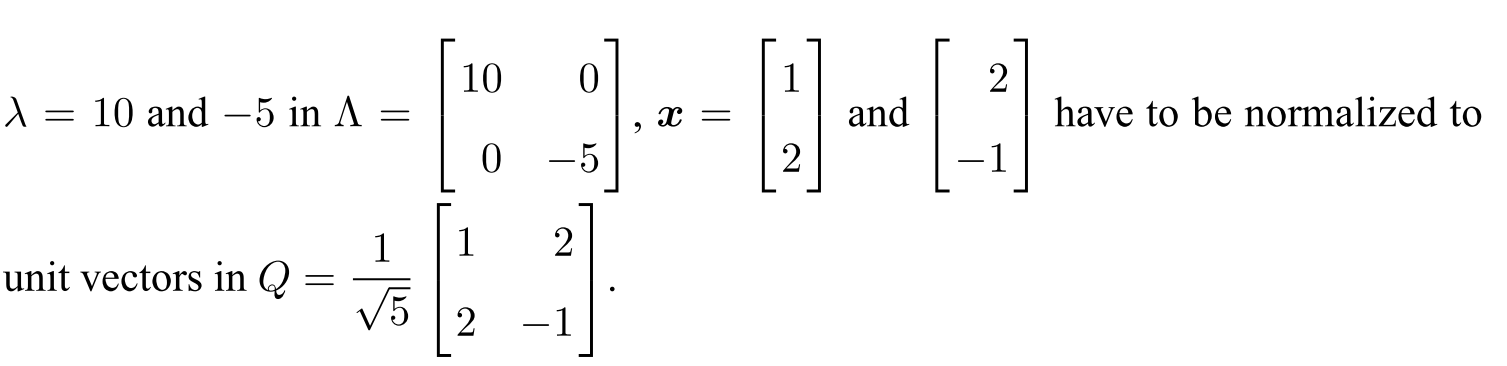
\includegraphics[height=1.5cm,width=1\textwidth,keepaspectratio]{2ans.png}
            % \caption{caption_name}
            \label{fig:2ans.png}
        \end{figure}
    }
\end{frame}

\begin{frame}[t]{Task 3}
    \framesubtitle{}
    \begin{figure}[H]
        \centering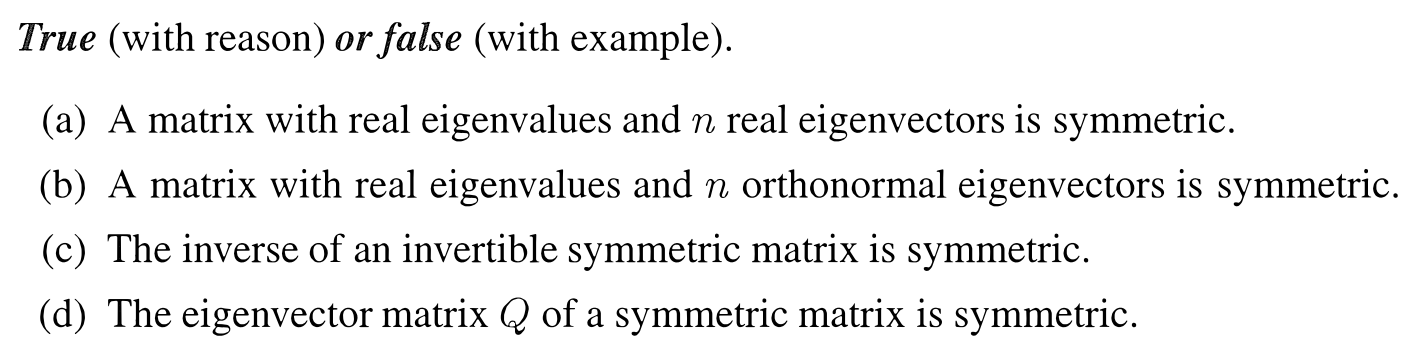
\includegraphics[height=3cm,width=1\textwidth,keepaspectratio]{3.png}
        % \caption{caption_name}
        \label{fig:3.png}
    \end{figure}
    \uncover<2->{
        \alert{\Large Answer}
        \begin{figure}[H]
            \centering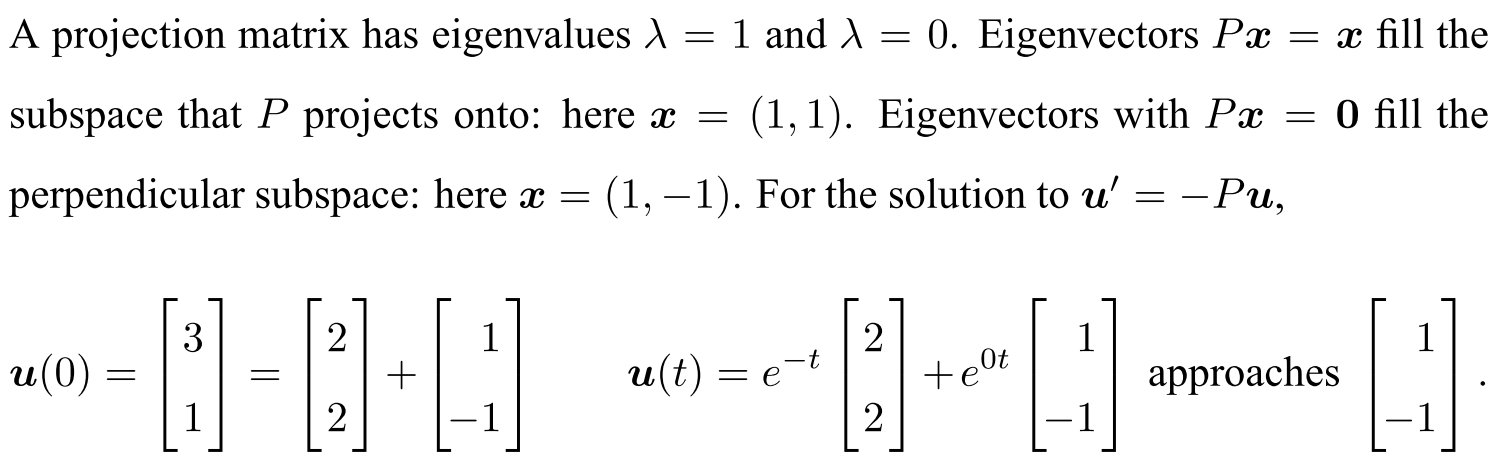
\includegraphics[height=3cm,width=1\textwidth,keepaspectratio]{3ans.png}
            % \caption{caption_name}
            \label{fig:3ans.png}
        \end{figure}
    }
\end{frame}

\begin{frame}[t]{Task 4}
    \framesubtitle{}
    \vspace{-0.5cm}
    \begin{figure}[H]
        \centering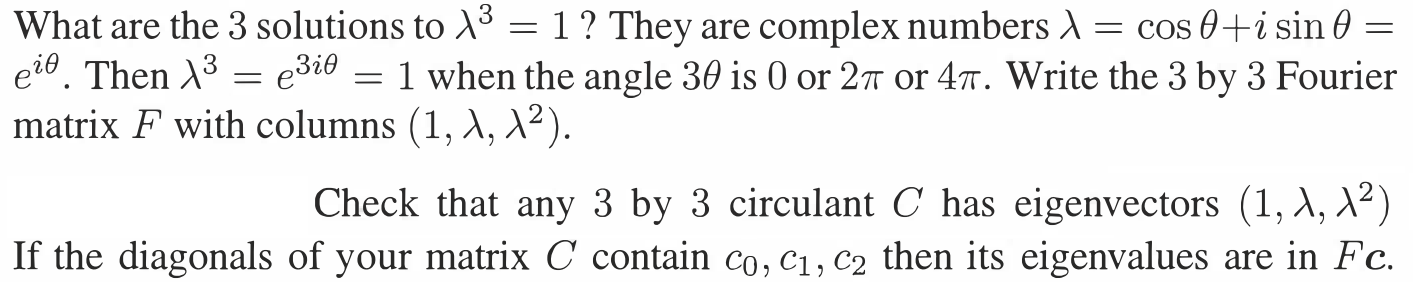
\includegraphics[height=3cm,width=1\textwidth,keepaspectratio]{1.png}
        % \caption{caption_name}
        \label{fig:1.png}
    \end{figure}
    \uncover<2->{
        \alert{\Large Answer}
        \begin{figure}[H]
            \centering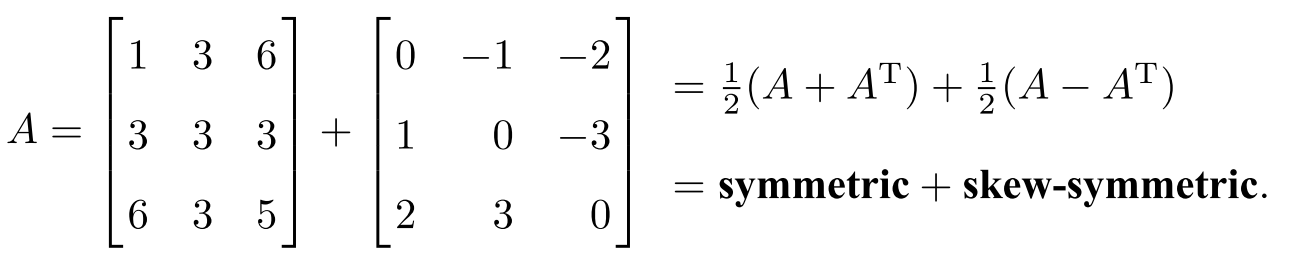
\includegraphics[height=3cm,width=1\textwidth,keepaspectratio]{1ans.png}
            % \caption{caption_name}
            \label{fig:1ans.png}
        \end{figure}
    }
\end{frame}


\begin{frame}[t]{Circulant Matrix}
\framesubtitle{}
\vspace{-0.4cm}
\textit{Watch first video on page \ref{itm:circulant}, if you want to look at derivation and the necessity of the matrix. }
\vspace{-0.2cm}

\textbf{Circulant matrix ($N=4$) is:}
\begin{equation*}
    C_4 = c_0I+ c_1P + c_2P^2 + C_3P^3 = \begin{bmatrix}
    c_0 & c_1 & c_2 & c_3\\
    c_3 & c_0 & c_1 & c_2 \\ 
    c_2 & c_3  & c_0 & c_1 \\
    c_1 & c_2  & c_3 & c_0 
    \end{bmatrix}, \text{ where } P = \begin{bmatrix}
    0 & 1 & 0 & 0\\
    0 & 0 & 1 & 0 \\ 
    0 & 0  & 0 & 1 \\
    1 & 0  & 0 & 0 
    \end{bmatrix}
\end{equation*}
\textbf{Properties:} \\ 
It has \textbf{\textit{eigenvectors}} in the Fourier Matrix columns $F_4 = \begin{bmatrix}
1 & 1 & 1 & 1\\
1 & i & -1 & -i \\ 
1 & i^2  & 1 & (-i)^2 \\
1 & i^3  & -1 & (-i)^3 
\end{bmatrix}$ \\

\textit{\textbf{Eigenvalues}} of $C$ can be found by Fourier trans. $F_4[c_0,\ c_1,\ c_2,\ c_3]^T = [\lambda_0,\ \lambda_1,\ \lambda_2,\ \lambda_3]^T$
\end{frame}

\begin{frame}[t]{Circulant Matrix}
\framesubtitle{Example}
    \begin{figure}[H]
        \centering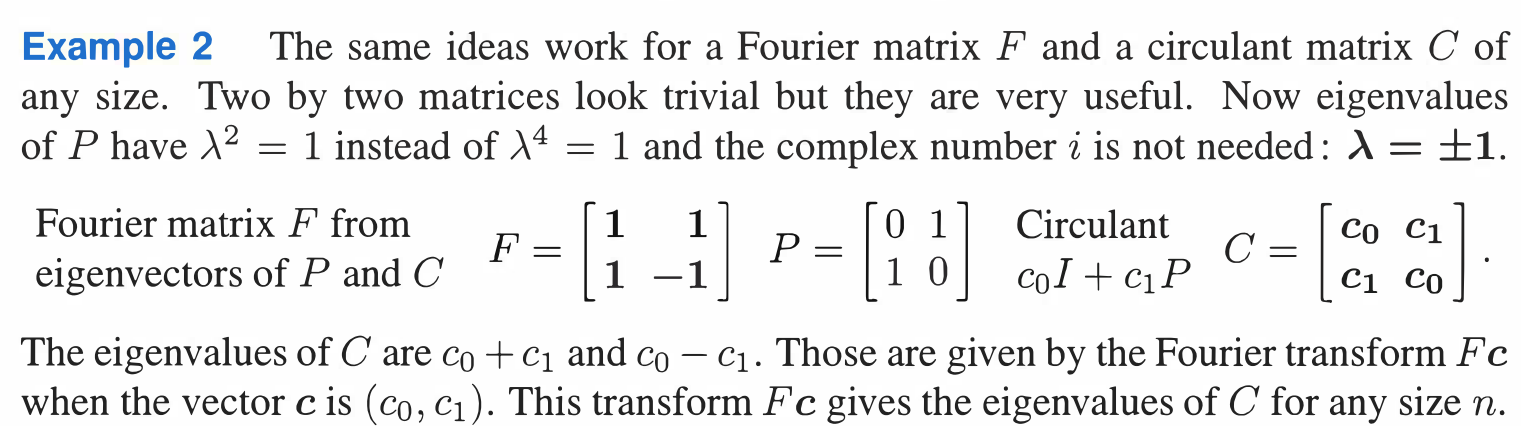
\includegraphics[height=6cm,width=1\textwidth,keepaspectratio]{circ_22.png}
        % \caption{caption_name}
        \label{fig:circ_22.png}
    \end{figure}
\end{frame}

\note{Эта тема на тестах у них была все время. Поэтому она тут.

Сделать упор, на то, что если они хотят понять смысл -- посмотреть видео Стренга.

Я на доске расписывал прям что на доске написано. Объяснял как записывать матрицу самому (каждая новая строка имеет последний элемент предыдущей и потом остальные в том же порядке что и наверху.)

Потом решали руками 2 на 2 и проверяли через классику(решение через собственные числа, а потом что получится при применении свойства.)

Разбирали, что если не понял тему фурье, то надо в читшит записать себе $F_{1-4}$, так как выше не будет 90 процентов}

\begin{frame}[t]{Task 5}
    \framesubtitle{}
    \vspace{-0.3cm}
    \only<1>{
    \begin{figure}[H]
        \centering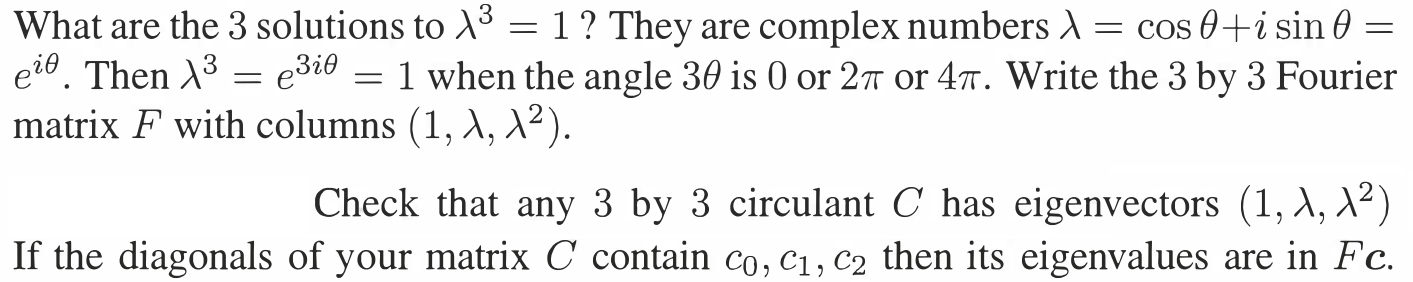
\includegraphics[height=5cm,width=1\textwidth,keepaspectratio]{1_rec.png}
        % \caption{caption_name}
        \label{fig:1_rec.png}
    \end{figure}
    }
    \only<2>{
        \alert{\Large Answer}
        \vspace{-1cm}
        \begin{figure}[H]
            \centering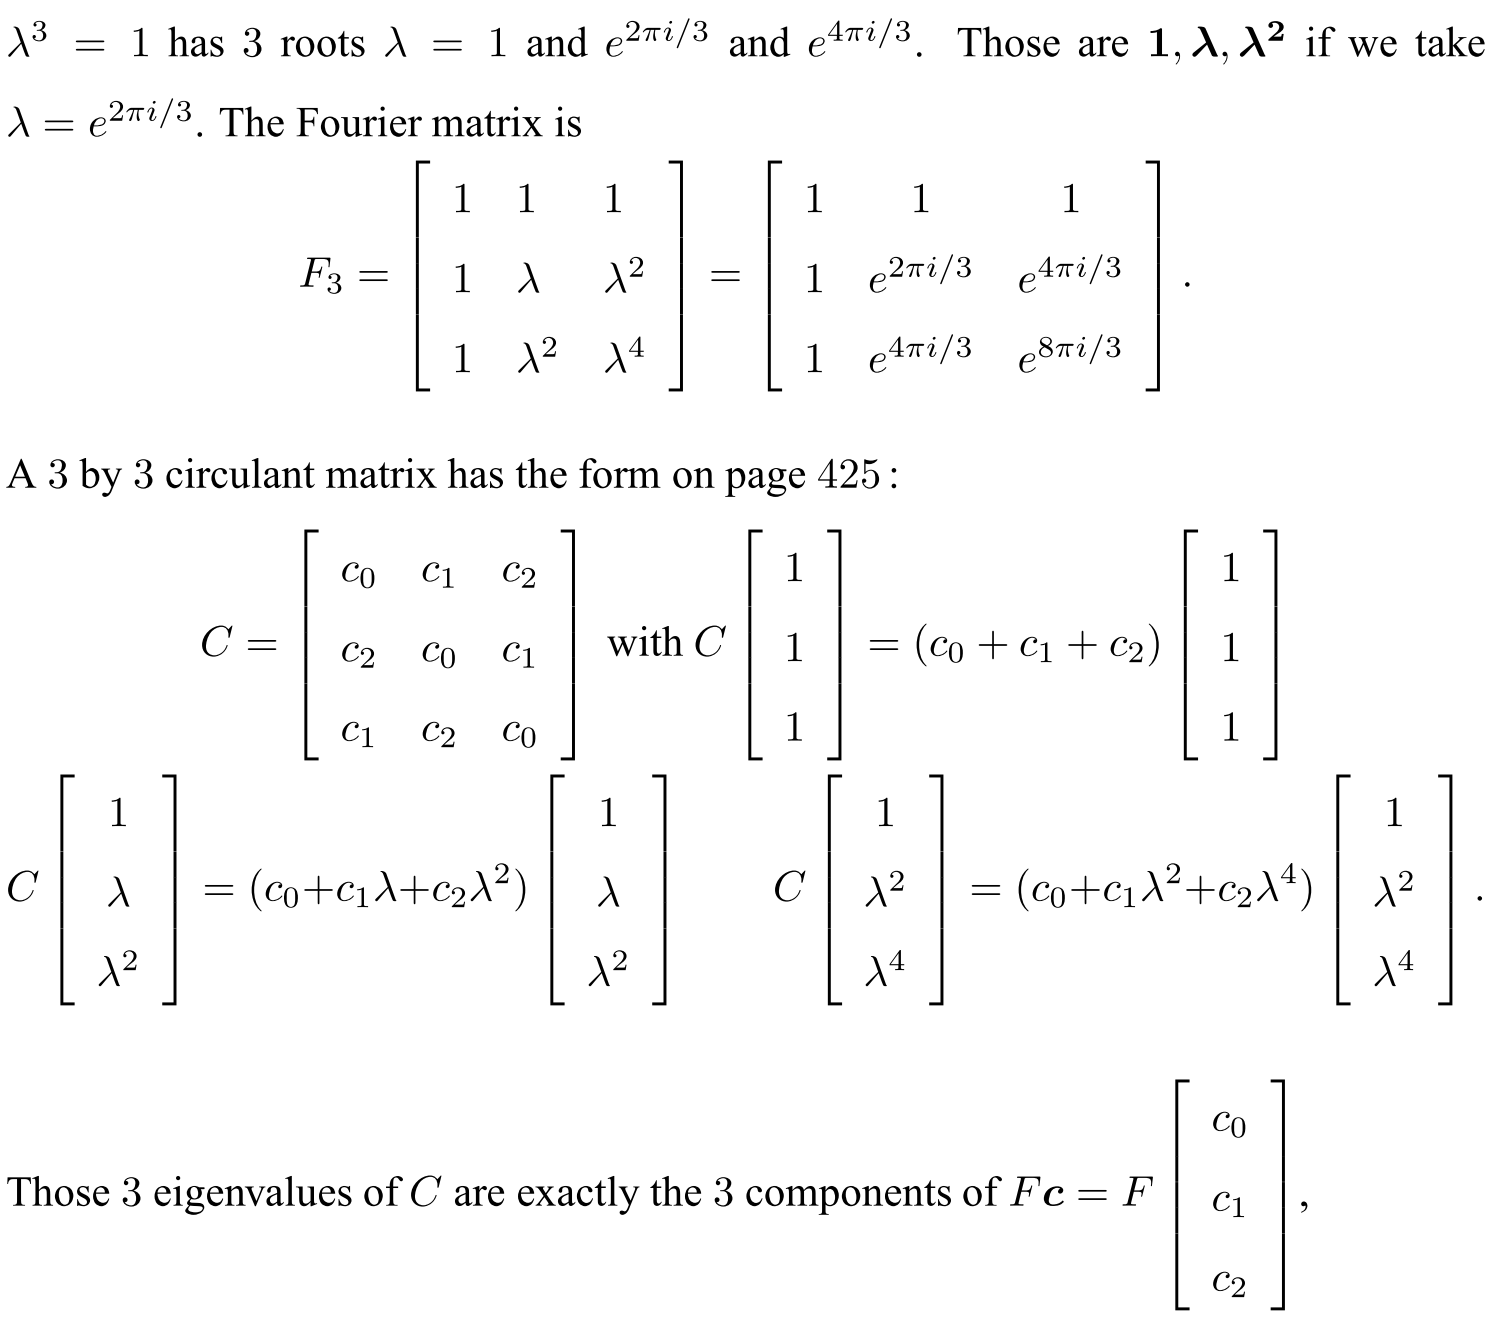
\includegraphics[height=7cm,width=1\textwidth,keepaspectratio]{1ans_rec.png}
            % \caption{caption_name}
            \label{fig:1ans_rec.png}
        \end{figure}
    }
\end{frame}

\note{Задачка простая, по факту делаем теперь 3 на 3. Но написано сложно. Поэтому и была добавлена, чтобы научились читать страшые текста.}

\begin{frame}[t]{Reference material}
    \framesubtitle{}
    \vspace{-0.6cm}
    \Large
    \begin{itemize}
        \item \href{https://youtu.be/vA9dfINW4Rg}{Fourier Series}
        \item \href{https://www.youtube.com/watch?v=M0Sa8fLOajA&list=PL49CF3715CB9EF31D&index=27}{Lecture 26, 2nd part}
        \item \textit{"Linear Algebra and Applications", pdf pages 221--234 }\\ Fast Fourier Transform
        \item \textit{"Introduction to Linear Algebra", pdf pages 456--462 }\\ Fast Fourier Transform
        \item  \textit{"Introduction to Linear Algebra", pdf pages 501--506 }\\ Fourier Series:  Linear Algebra for Functions 
        \item \href{https://youtu.be/1pFv7e9xtHo}{Eigenvectors of Circulant Matrices: Fourier Matrix} \label{itm:circulant}
    \end{itemize}
\end{frame}

\fbckg{fibeamer/figs/last_page.png}
\frame[plain]{}

\end{document}